\documentclass[a4paper,12pt]{article}  

\usepackage[utf8]{inputenc}  
\usepackage{amsmath}         
\usepackage{graphicx}        

\title{Model za prepoznavanje stopnje prizadetosti s pomočjo testa tapkanja s prsti pri bolnikih s 
Parkinsonovo boleznijo \\ 
Predstavitev magistrskega dela}
\author{Neža Kržan \\
Mentor: doc. dr. Jure Žabkar}          

\usepackage{float}       
\usepackage{graphicx}
\usepackage[slovene]{babel}
\usepackage{float}
\usepackage[T1]{fontenc}
\usepackage{pdflscape}
\usepackage{adjustbox}
\usepackage{graphicx}
\usepackage{booktabs}
\usepackage{longtable}
\usepackage{array}
\usepackage{bookmark}
\usepackage[backend=biber, style=numeric]{biblatex}
\usepackage[a4paper,margin=1in]{geometry}
\usepackage{csquotes}

\addbibresource{literatura.bib}

\begin{document}
\maketitle

%%%%%%%%%%%%%%%%%%%%%%%%%%%%%%%%%%%%%%%%%%%%%%%%%%%%%%%%%%%%%%%%%%%%%%%%%%%%%%%%%%%%%%%%%%%%%%%%%%%%%
\section{Parkinsonova bolezen}

Parkinsonova bolezen je kronična, nevrodegenerativna motnja osrednjega živčnega sistema, ki vpliva 
predvsem na gibanje. Nastane zaradi postopnega propadanja dopaminergičnih nevronov v substanci 
nigra (\textit{lat. substantia nigra}) v delu možganov, ki vpliva na motorične sposobnosti, spanje, vedenje, 
razpoloženje, zbranost, zaznavanje, itd. \
Glavni simptomi so tremor oz. tresenje, bradikinezija, togost mišic (rigidnost) in nestabilnost (moteni posturalni refleksi). 
Poleg težav z motoričnostjo pojavijo tudi drugi simptomi, kot so depresija, 
motnje spanja, kognitivni upad in avtonomna disfunkcija. Tem simptomom se velikokrat priklučijo tudi 
atipični simptomi, npr. ataksija (kaže se kot neusklajenost gibov)~\cite{NINDS}. \\

Bolezen napreduje postopoma in trenutno ni ozdravljiva, vendar se simptomi lahko obvladujejo z zdravili 
in v nekaterih primerih s kirurškim postopkom globoke možganske električne stimulacije~\cite{Sveinbjornsdottir}. 
Pogosto se za ocenjevanje napredovanja bolezni in spremljanje njenega napredovanja uporablja lestvica 
MDS-UPDRS (\textit{Movement Disorder Society-Unified Parkinson's Disease Rating Scale}). Ocenjevanje temelji na 
nevroloških pregledih v ambulanti, kjer pacient izvaja motorične naloge~\cite{Goetz}. \\

\subsection{Testi za diagnosticiranje in spremljanje Parkinsonove bolezni}

Obstaja več različnih testov za diagnosticiranje in spremljanje Parkinsovove bolezni, ki ocenjujejo 
motorične in nemotorične simptome.\
Glavna in standardna lestvica za ocenjevanje napredovanja bolezni je MDS-UPDRS, na podlagi katere so 
podane tudi ocene naših bolnikov. Široko uporabljena je tudi lestvica Hoehn in Yahr, ki razvršča 
bolezen v 5 stopenj glede na resnost simptomov~\cite{Bhidayasiri, wiki}.\
Med pregledom se izvajajo različni motorični testi - med najbolj pogostimi so preverjanje ravnotežja, 
test hoje in tapkanje s prsti (\textit{angl. finger tapping}).\
Obstajajo tudi psihološki testi za zgodnje odkrivanje kognitivnih motenj, oceno spomina, orientacijo, 
pozornost in spremljanje depresije. Ponavadi pacienta napotijo tudi na MRI ali CT glave. Obstajajo 
tudi nosljive naprave, ki merijo tremor, gibanje in posturalno stabilnost.

\subsection{Test tapkanja}

Za ocenjevanje stopnje bolezni se najpogosteje uporablja standardizirana lestvica MDS-UPDRS. Sestavljena je 
iz štirih delov:

\begin{enumerate}
    \item nemotorične izkušnje v vsakdanjem življenju,
    \item motorične izkušnje v vsakdanjem življenju,
    \item pregled motoričnih sposobnosti,
    \item zapleti zdravljenja motoričnih simptomov.
\end{enumerate}

Deli so ovrednoteni po lestvici od 0 do 4, kot kaže tabela \ref{table:mds_updrs}.\\

V posameznem sklopu je več različnih vrst testov ali vprašanj, v sklopu ocenjevanja motoričnih sposobnosti pa je 
tudi test tapkanja s prsti s pomočjo katerega ocenjujemo stopnjo bradikinezije. \
Test poteka tako, da testiranec s kazalcem najprej dotakne palca, nato pa ga čim bolj odmakne in ponovno vrne 
v začetni položaj. Vsak takšen gib predstavlja en cikel. Cilj je izvesti čim več ciklov v določenem časovnem 
obdobju (npr. 10 sekund) ali opraviti določeno število ciklov (npr. 10 do 15 ponovitev) s čim večjo hitrostjo in 
natančnostjo. Ocenjuje se hitrost (število tapkanj v določenem času), enakomernost gibov, prisotnost 
motenj (upočasnitev, tresenje, nepravilni gibi) in upad amplitude. Test je sicer preprost ampak subjektiven, 
kar predstavlja problem, saj je ovrednotenje odvisno od nevrologa. Le ta mora spremljati pozorno in 
prepoznati kakršno koli motnjo v gibanju, sicer lahko poda napačno oceno. Test se izvaja z obema rokama in 
samo enkrat med pregledom, saj ponovni test, zaradi možne utrujenosti pacienta, kar vpliva na motnje v 
gibanju, ni nujno reprezentativen~\cite{Goetz, Khana}. 

\begin{table}[H]
    \centering
    \renewcommand{\arraystretch}{1.3} % Doda več prostora med vrsticami
    \begin{longtable}{|c|p{12cm}|}
        \hline
        \multicolumn{2}{|c|}{\textbf{MDS-UPDRS tapkanje s prsti}} \\
        \hline
        \textbf{Ocena} & \textbf{Navodila za točkovanje} \\
        \hline
        \endfirsthead

        \hline
        \textbf{Ocena} & \textbf{Navodila za točkovanje} \\
        \hline
        \endhead

        0 & - brez težav \\
        \hline
        1 & - običajen ritem tapkanja prekinjen z 1-2 prekinitvama ali zakasnitvama tapkanja \\ 
          & - rahla upočasnitev hitrosti tapkanja \\ 
          & - upad amplitude proti koncu 10. cikla \\
        \hline
        2 & - običajen ritem tapkanja prekinjen s 3-5 prekinitvami ali zakasnitvami tapkanja \\ 
          & - blaga upočasnitev hitrosti tapkanja \\ 
          & - upad amplitude proti sredini 10. cikla \\
        \hline
        3 & - več kot 5 prekinitev med tapkanjem ali vsaj ena daljša zakasnitev tapkanja \\ 
          & - zmerna upočasnitev hitrosti tapkanja \\ 
          & - upad amplitude po 1. ciklu \\
        \hline
        4 & - naloge ni zmožen opraviti ali pa jo opravi s težavo zaradi upočasnitve \\ 
          & - prekinitev ali zmanjšanja amplitude in hitrosti \\
        \hline
    \end{longtable}
    \caption{Merila točkovanja po lestvici MDS-UPDRS za ocenjevanje naloge tapkanja s prsti. Nevrolog ocenjuje na 
    podlagi vsaj desetih ciklov odpiranja in zapiranja prstov, vsako roko ločeno. Ocenjuje se upad hitrosti in 
    amplitude ter prekinitve oziroma zakasnitve~\cite{Stamatakis}.}
    \label{tab:mds_updrs}
\end{table}

%%%%%%%%%%%%%%%%%%%%%%%%%%%%%%%%%%%%%%%%%%%%%%%%%%%%%%%%%%%%%%%%%%%%%%%%%%%%%%%%%%%%%%%%%%%%%%%%%%%%%
%%%%%%%%%%%%%%%%%%%%%%%%%%%%%%%%%%%%%%%%%%%%%%%%%%%%%%%%%%%%%%%%%%%%%%%%%%%%%%%%%%%%%%%%%%%%%%%%%%%%%
\section{Sorodna dela}
Različna dela proučujejo različne znake Parkinsonove bolezni, vendar med najpogosteje preučevanimi je 
tapkanje s prsti (\textit{finger tapping}), sledi ji gibanje rok (\textit{hand movements}), pronacija-supinacija 
(\textit{pronation-supination}) in tremor. Pogosto so tapkanje s prsti, gibanje rok in pronacija-supinacija 
preučevane skupaj, ker naj bi bile celoten pokazatelj ocene MDS-UPDRS~\cite{Manzanera}. \\

Študije sledijo kliničnim ciljem - stadij bolezni (ocena po MDS-UPDRS), prepoznavanje bolezni v primerjavi z 
zdravimi kontrolnimi primeri in ocena specifičnih simptomov (oceno tremorja, bradikinezije); največ študij 
se ukvarja z oceno bolezni po MDS-UPDRS in primerjavo značilk z zdravo kontrolno skupino~\cite{Amo-Salas}.\
Ocenjevanje telesnih gibov (\textit{HPE – Human Pose Estimation}) celotnega telesa je doseglo izjemno natančnost, 
sledenje gibom rok pa zaenkrat še predstavlja izzive. Podobno kot pri ocenjevanju telesnih gibov, tudi pri 
sledenju rok uporabljajo različne pristope - uporaba nosljivih naprav (IMU, senzorske rokavice) in uporaba 
računalniškega vida~\cite{Amprimoa}. \\

Algoritmi oziroma arhitekture, ki so jih izdelali v študijah vsebujejo različne načine obdelovanja posnetkov. V 
posnetkih sledijo gibanju rok oz. oceni pozicije roke s pomočjo različnih orodij (MediaPipe Hand, OpenPose, 
DeepLabCut in MMPose), obstajajo pa tudi primeri ko so uporabili globoko nevronsko mrežo neposredno na 
videoposnetkih tapkanja s prsti.\
Večina uporablja nabor sklepov modela roke COCO (\textit{angl. COCO Hand model}). \\

Identificirali so posamična gibanja tapkanja s prsti - cikel tapkanja z izračunom razdalje med palcem in 
kazalcem oz. kotne razdalje med palcem in kazalcem in tako določili vrh in dno amplitude oz. odpiranje in 
zapiranje prstov. Večina se jih je posluževalo izračuna evklidske razdalje med palcem in kazalcem, saj so 
bili koti občutljivi na nagib kamere.  \\

Večina avtorjev je svoje modele gradila na ročno izračunanih značilkah (\textit{angl. manual features}) glede na 
smernice ocen po lestvici MDS-UPDRS (glede na to kaj se ocenjuje pri posamezni oceni). Ker pa nekateri 
niso dobro poznali problema in značilnosti Parkinsonove bolezni, ali pa so model, naučen na ročno izračunanik 
značilkah, želeli primerjati, so se izračuna značilk lotili z nevronskimi mrežami. \
Ročni izračun značilk je temeljil na pospešku (\textit{angl. acceleration}), kotni hitrosti (\textit{angl. angular velocity}), 
premiku (\textit{angl displacement}) in kotu (\textit{angl. angle}) v časovni vrsti oz. amplitudah. Glede na vrhove amplitud 
so računali še število gibanj, štetih po maksimalnih vrhovih, maksimalen vrh in dno ter minimalen vrh in dno 
amplitude, povprečno število maksimalnih in minimalnih vrhov ter dna glede na določen časovni interval ter 
število vrhov v določenem časovnem intervalu. Nekateri so v model vključili tudi dva demografska dejavnika, 
spol in starost. \\

Večina je zgradila en sam večrazredni klasifikacijski model, kar pomeni, da izhod modela predstavlja vse 
ocene po lestvici MDS-UPDRS. Nekateri pa so uporabljali več binarnih klasifikatorjev. Gradili so različne 
modele, med najbolj pogostimi pa so bili metoda podpornih vektorjev (\textit{angl. Support Vector Machine}), naključni 
gozdovi (\textit{angl. Random Forest}) in XBoost ter običajni klasifikatorji, kot so odločitvena drevesa (\textit{angl. Decision 
Tree}), model $k$-najbližjih sosedov (\textit{angl. $k$-nearest neighbors}) in logistična regresija (\textit{logistic 
regression}). \
Pri iskanju so uporabljali le podatke za učenje, da bi dodatno 
zagotovili robustnost naučenih klasifikatorjev oz. modelov. Podatki so torej bili razdeljeni na učne in 
testne, ponavadi v razmerju 70\%/30\% ali 80\%/20\%, modeli pa preverjeni z $k$-kratnom navzkrižnim 
preverjanjem (\textit{angl. $k$ - Cross Validation}), v večini primerov $k$ = 5, nekje celo $k$ = 10.\
Za vrednotenje modelov so standardno uporabljali štiri različne metrike, točnost (\textit{angl. accuracy}), 
natančnost (\textit{angl. precision}), priklic (\textit{angl. recall}) in F1. Pogosto je bila primerjava modelov narejena 
tudi na podlagi ploščine pod krivuljo (\textit{angl. Area Under Curve}). 

%%%%%%%%%%%%%%%%%%%%%%%%%%%%%%%%%%%%%%%%%%%%%%%%%%%%%%%%%%%%%%%%%%%%%%%%%%%%%%%%%%%%%%%%%%%%%%%%%%%%%
%%%%%%%%%%%%%%%%%%%%%%%%%%%%%%%%%%%%%%%%%%%%%%%%%%%%%%%%%%%%%%%%%%%%%%%%%%%%%%%%%%%%%%%%%%%%%%%%%%%%%
\section{Motivacija}

Ker natančna in zgodnja klasifikacija stopnje Parkinsonove bolezni omogoča pravočasno zdravljenje in 
prilagoditev terapije, bi razvoj dobrega klasifikacijskega modela za prepoznavanje stopnje Parkinsonove 
bolezni po lestvici MDS-UPDRS zelo pripomogel k boljšemu spremljanju bolnikov. Napovedovanje stopnje 
bradikinezije na podlagi testa tapkanja s prsti je mogoče že nekaj časa z uporabo senzorjev, kar sicer ni 
dostopno vsem. Želimo si razviti klasifikacijski model, ki bo čim bolj natančno, na podlagi posnetkov tapkanja 
s prsti posnetih v ambulanti, lahko določil stopnjo bradikinezije Parkinsonove bolezni po lestvici MDS-UPDRS.

%%%%%%%%%%%%%%%%%%%%%%%%%%%%%%%%%%%%%%%%%%%%%%%%%%%%%%%%%%%%%%%%%%%%%%%%%%%%%%%%%%%%%%%%%%%%%%%%%%%%%
%%%%%%%%%%%%%%%%%%%%%%%%%%%%%%%%%%%%%%%%%%%%%%%%%%%%%%%%%%%%%%%%%%%%%%%%%%%%%%%%%%%%%%%%%%%%%%%%%%%%%
\section{Podatkovna zbirka}

Videoposnetki tapkanja so bili posneti z različnimi pametnimi telefoni, nekateri pri hitrosti 30 sličic na 
sekundo, večina pa pri 60 sličicah na sekundo. Ločljivost snemanja je bila 3840$\times$2160 slikovnih pik, pri 
nekaterih pa 1920$\times$1080 slikovnih pik. Posnetki so bili zajeti v različnih okoljih in ni nujno, da je bila 
kamera postavljena pravokotno na profil palca in kazalca. Tudi osvetlitve med posnetki se razlikujejo, razdalje 
med kamero in roko pa so različne. Posnetki so bili za potrebe analize obrezani tako, da je na njih vidna 
celotna roka in manj okolice, kar nam omogoča hitrejše procesiranje ter izvedbo analize na manj 
zmogljivih sistemih, zaradi manjšega števila slikovnih pik videa. Odstranjeni so bili posnetki, kjer 
celotna roka ni bila vidna, ter posnetki, kjer so koti snemanja močno odstopali od pravega kota, ker so 
povzročali težave pri zaznavi roke. \
Večino videov je bilo zajetih od pacientov s Parkinsonovo boleznijo v ambulanti na Univerzitetnem kliničnem 
centru v Ljubljani, nekaj pa od prostovoljcev v različnih okoljih. Odstranjeni so bili tudi posnetki udeležencev, ki 
niso imeli potrjene Parkinsonove bolezni vendar pa so po lestvici MDS-UPDRS dobili oceno višjo od nič. \
Zbranih je bilo 183 posnetkov 91 različnih posameznikov. Stopnjo motorične prizadetosti v posnetkih je po 
lestvici MDS-UPDRS od 0 do 4 ocenil nevrolog. Za vsakega udeleženca sta bila pridobljena dva posnetka, enega 
iz tapkanje leve roke in drugega iz tapkanja desne roke. Pri določanju stopnje motorične prizadetosti na 
podlagi testa tapkanja se je ocenjevala dominantna roka~\cite{Zupanic}. 

%%%%%%%%%%%%%%%%%%%%%%%%%%%%%%%%%%%%%%%%%%%%%%%%%%%%%%%%%%%%%%%%%%%%%%%%%%%%%%%%%%%%%%%%%%%%%%%%%%%%%
\subsection{Predprocesiranje podatkov}

Posnetki so obrezani, da odstranimo čim več slikovnih pik okolice, ki ne zajemajo območja roke. Na posnetkih 
sta uporabljena orodja Mediapipe Hand in MMpose. Mediapipe Hand naj ne bi v določenih primerih zaznal pozicije prstov 
oziroma naj bi zamenjal palec in sredinec. Razlike med MediaPipe Hand zaznavo roke in MMPose bomo ugotavljali. \\

MediaPipe Hand in MMPose orodje uporablja nabor sklepov modela roke COCO (\textit{angl. COCO Hand model}). Model roke 
je setsavljen iz 21 točk, ki predstavljajo glavne sklepe roke~\cite{Li1}. \\

\begin{figure}[H]
  \centering
  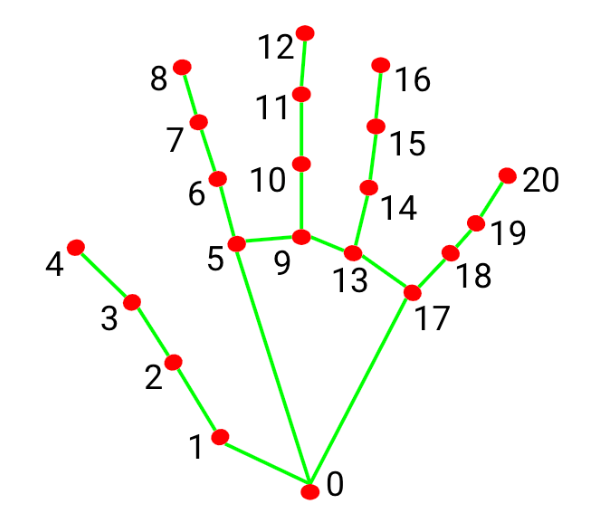
\includegraphics[width=0.7\textwidth]{slike/coco_hand.png}  
  \caption{COCO Hand model, tipična konfiguracija sklepov v orodju MediaPipe Hand in MMPose~\cite{Li1}.}
  \label{fig:coco_hand}
\end{figure}

Iz dobljenih skeletov izračunamo evklidske razdalje med končnimi točkami palca in kazalca (točki 4 in 8 na 
sliki~\ref{fig:coco_hand}) in 
med točkami zadnjih sklepov palca in kazalca (točki 3 in 7 na sliki~\ref{fig:coco_hand}). \
Namesto evklidske razdalje bi lahko izračunali kote med palcem in kazalcem, ampak zaradi različnih 
načinov snemanja je prihajalo do nagibov kamere, kar pomeni, da kot med roko in kamero ni nujno 90 stopinj. 
Koti so sicer neodvisni od razdalje med kamero in roko, ampak so veliko bolj občitljivi na kot snemanja, 
zato je evklidska razdalja boljša izbira. \\

Zaradi primerjave med orodjema MediaPipe Hand in MMPose in zaradi različnih razdalj med kamero in roko smo na 
amplitudah izvedli min-max normalizacijo.

\begin{figure}[H]
  \centering
  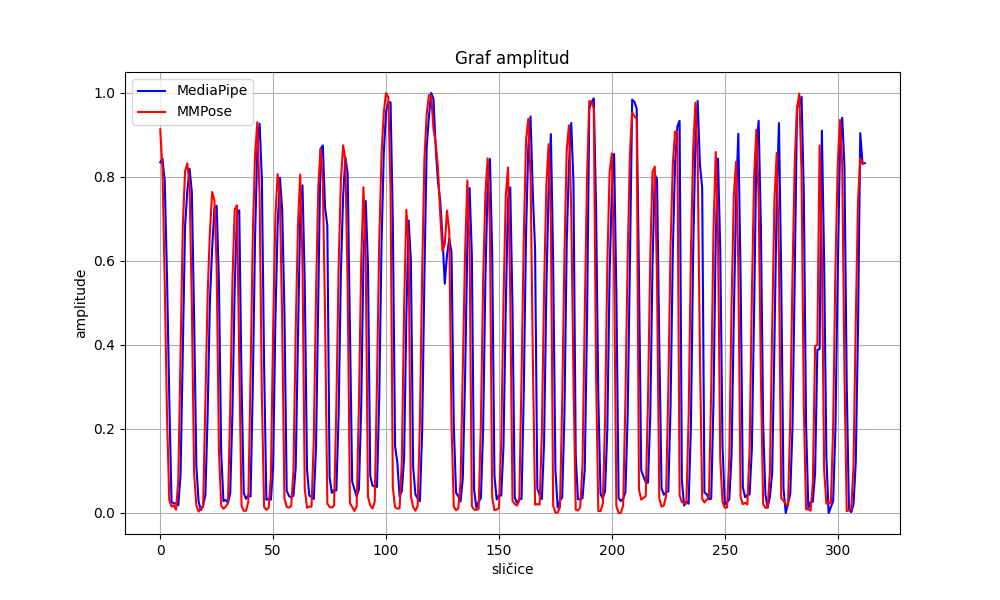
\includegraphics[width=0.8\textwidth]{slike/distances_plot_both.png}  
  \caption{Graf amplitude pridobljenih z evklidsko razdaljo med konicama palca in kazalca iz skeleta orodij MediaPipe Hand in MMPose.}
  \label{fig:amplituda_oba}
\end{figure}

%%%%%%%%%%%%%%%%%%%%%%%%%%%%%%%%%%%%%%%%%%%%%%%%%%%%%%%%%%%%%%%%%%%%%%%%%%%%%%%%%%%%%%%%%%%%%%%%%%%%%
\subsection{Analiza podatkov}

Ker bomo v sklopu naloge raziskovali tudi natančnost klasifikatorja stopnje motorične prizadetosti po MDS-UPDRS, 
bomo verjetno uporabili tapkanje obeh rok enega udeleženca, ker je tapkanje leve in desne roke med seboj neodvisno.\\

Posnetki so pridobljeni za vseh 5 ocen po lestvici MDS-UPDRS (torej imamo tudi kontrolno skupino), od 183 posnetkov 
imamo pri 88 video posnetkih zabeležen spol. Imamo 46 posnetkov, kjer je zabeležen moški spol in 42 posnetkov, kjer
je zabeležen ženski spol.

\begin{table}[H]
  \centering
  \renewcommand{\arraystretch}{1.3} 
  \begin{longtable}{|l|c|c|c|c|c|c|}
      \hline
      \multicolumn{7}{|c|}{\textbf{Število video posnetkov in delež po MDS-UPDRS ocenah}} \\
      \hline
      \textbf{Ocena MDS-UPDRS} & \textbf{0} & \textbf{1} & \textbf{2} & \textbf{3} & \textbf{4} & \textbf{Skupaj} \\
      \hline
      Moški & 12 & 11 & 1  & 8  & 3  & 46 \\
      Delež moških & 26\% & 24\% & 26\% & 17\% & 7\%  & 100\% \\
      Ženske & 14 & 10 & 13 & 5  & 0  & 42 \\
      Delež žensk & 33\% & 24\% & 31\% & 12\% & 0\%  & 100\% \\
      Skupno število video posnetkov & 29 & 51 & 53 & 23 & 7  & 183 \\
      Delež & 26\% & 28\% & 29\% & 13\% & 4\%  & 100\% \\
      \hline
  \end{longtable}
  \caption{Število video posnetkov in delež, kjer je bil zabeležen spol in število video posnetkov testa tapkanja 
  po ocenah MDS-UPDRS in njihovi deleži.}
  \label{tab:video_posnetki}
\end{table}

Razlike med amplitudami glede na oceno po lestvici MDS-UPDRS lahko vidimo na spodnjih grafih. \\

\begin{figure}[H]
  \centering
  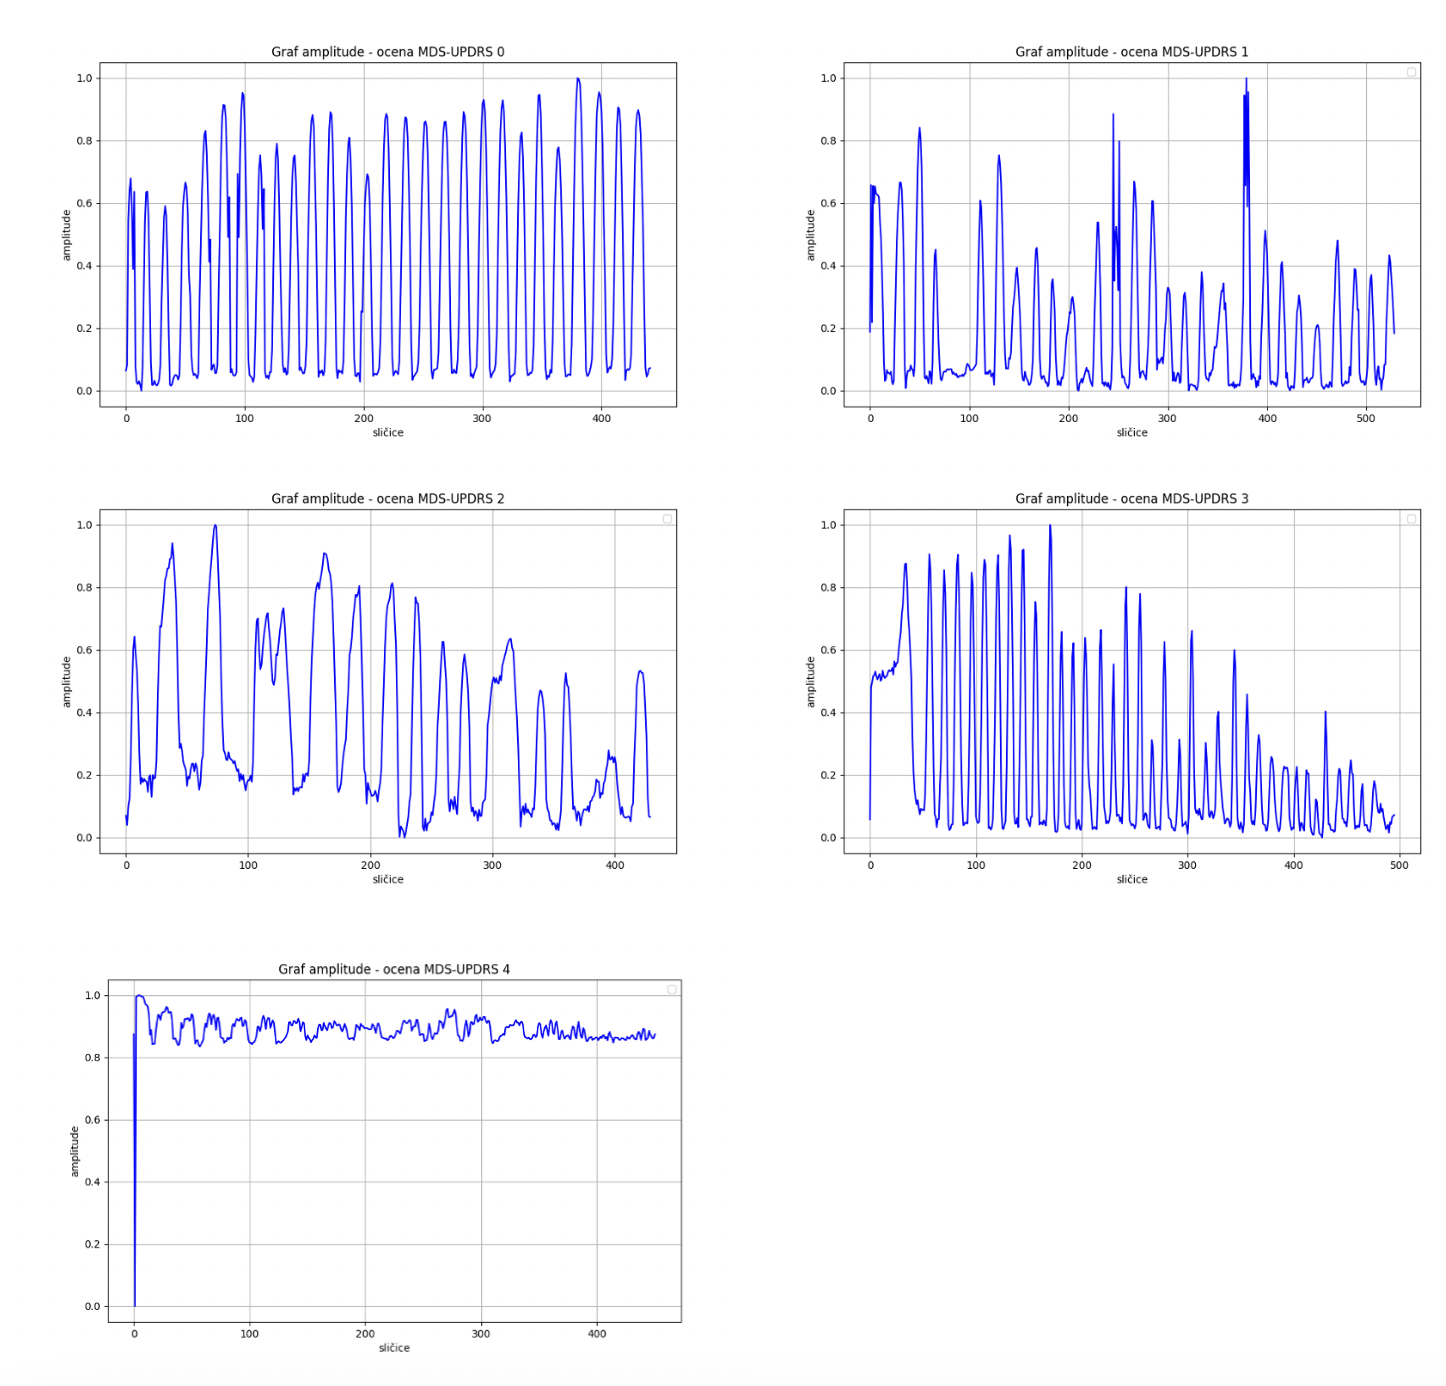
\includegraphics[width=0.9\textwidth]{slike/ocene.png}  
  \caption{Grafi amplitud pridobljenih z evklidsko razdljo med konicama palca in kazalca iz skeleta orodij 
  MediaPipe Hand za vseh 5 ocen MDS-UPDRS.}
  \label{fig:amplitude_ocene}
\end{figure}

%%%%%%%%%%%%%%%%%%%%%%%%%%%%%%%%%%%%%%%%%%%%%%%%%%%%%%%%%%%%%%%%%%%%%%%%%%%%%%%%%%%%%%%%%%%%%%%%%%%%%
%%%%%%%%%%%%%%%%%%%%%%%%%%%%%%%%%%%%%%%%%%%%%%%%%%%%%%%%%%%%%%%%%%%%%%%%%%%%%%%%%%%%%%%%%%%%%%%%%%%%%
\section{Potek dela}
V nalogi se želimo osredotočiti predvsem na ročno grajenje značilk (\textit{angl. features}) 
in gradnjo modelov. Cilj je razviti preprost in učinkovit model, ki ga bomo dobro razumeli. \\

Začeli smo s pregledom dosedanjih študij, kjer smo ugotovili, kaj je bil poudarek do sedaj in kaj si želimo 
narediti bolje. Pregledali smo posnetke, njihovo obdelavo in možnosti izboljšanja. Uporabili smo
orodje MediaPipe Hand in MMPose za prepoznavo roke in iz časovne vrste skeleta roke izračunali evklidske 
razdalje med končnimi točkami palca in kazalca. Na začetku se bomo lotili izračuna značilk in gradnje 
modelov z amplituadmi, pridobljenimi z orodjem Mediapipe Hand. \\

Razvoj zanačilk bi vseboval dobro opredelitev le-teh, zajem različnih značilk glede na naš problem in 
izbor najustreznejših, na podlgi katerih bi gradili model. V razvoj značilk bi lahko vključili tudi statistično 
analizo le-teh na podlagi ocen po lestvici MDS-UPDRS in tako ugotovili, katere značilke bolje opisujejo 
posamezne ocene. \\

Analiza gibanja prstov skozi krivulje nam omogoča vpogled v določene značilnosti motoričnih funkcij. Naš 
cilj je preveriti, ali lahko krivulje odražajo informacije, ki jih želimo pridobiti iz besedilnih opisov 
ocenjevanja po lestvici MDS-UPDRS. \
Najprej bi matematično definirali idealno krivuljo, ki opisuje optimalno gibanje tapkanja s prsti (kot kontrolna 
skupina). Ker imamo podatke o gibanju prstov zdravega posameznika (ocena po lestvici MDS-UPDRS je enaka 0), 
bi nam to omogočilo primerjavo in iskanje odstopanj/anomalij. Zanima nas ali lahko v teh krivuljah prepoznamo 
anomalije, ki jih znamo matematično opisati - amplituda, frekvenca in njihova nihanja. S prilagajanjem teh 
anomalij lahko generiramo amplitude, ki simulirajo različne hitrosti tapkanja s prsti, frekvenčne spremembe, zamrznitve gibanja 
ter postopno zmanjševanje oz. upad amplitude. Tako bi pridobili veliko količno podatkov, ki jih lahko 
analiziramo in uporabimo za učenje modelov za odkrivanje anomalij. Z umetno generiranimi amplitudami oz. podatki bi 
lahko povezali tekstovni opis ocene z oceno po lestvici MDS-UPDRS. Če uspemo model naučiti prepoznavanja 
anomalij, lahko na podlagi tega podamo tekstovni opis, ki bi služil kot diagnoza, za kar bi lahko uporabili jezikovne modele. S tem bi pridobili 
razlago, zakaj je model vrnil določeno oceno in zakaj je takšna, kot je. \\

Preprosti modeli, kot so metoda podpornih vektorjev, naključni gozdovi in model $k$-najbližjih sosedov, so 
v drugih študijah dosegali zelo dobre rezultate, ampak se študije niso osredotočale na gradnjo 
modelov, ampak predvsem na obdelavo video posnetkov oz. podatkov in na izračun nekaterih značilk. Zato si 
želimo v nalogi dobre razlage modela/modelov in poznavanje njegovega delovanja.

%%%%%%%%%%%%%%%%%%%%%%%%%%%%%%%%%%%%%%%%%%%%%%%%%%%%%%%%%%%%%%%%%%%%%%%%%%%%%%%%%%%%%%%%%%%%%%%%%%%%%
\newpage
\printbibliography

\end{document}